\documentclass{beamer}
\usepackage[utf8]{inputenc}
\usepackage[T1]{fontenc}

\usepackage{hyperref}
\usepackage{csquotes}
\usepackage[
	backend=biber,
	style=numeric,
	citestyle=numeric,
	sorting=none,
	url=false]{biblatex}

\setbeamertemplate{bibliography item}[text]
\renewcommand*{\bibfont}{\scriptsize}
\addbibresource{content/biblio.bib}


\usepackage{array}
\usepackage{tabularx}
\usepackage{lipsum}


\setcounter{tocdepth}{3}

\usepackage{bbold}
\usepackage{scalerel}[2016/12/29]

\newcolumntype{M}[1]{>{$\displaystyle\qquad}p{#1}<{$}}

\usepackage{appendixnumberbeamer}

\usepackage{graphicx}
\graphicspath{{Im/}}


\newcounter{FootlineChoice} 
% Counter to allow the user to choose between a few footlines implemented by owner

\newcounter{DepartmentLogo}
% Counter to allow the user to choose whether to display the Department Logo in NE corner

\newcounter{FacultyLogo}
% Counter to allow the user to choose whether to display the Faculty Logo in SE corner
\usetheme{ULB}

%%%%%%%%%%%%%%%%%%%%%%%%%%%%%%%%%%%%%%%%%%%%%%%%%%%%%%%%%%%%%%%%%%%%%%%%%%%%%%%%%%%%%%%%%%%%%%%%%%%%%%%%%%%%%%%%%%%%%%%%%%%%%
%%%%%%%%%%%%%%%%%%%%%%%%%%%%%%%%%%%%%%%%%%%%%%%%%%%%%% DEPARTMENT LOGO %%%%%%%%%%%%%%%%%%%%%%%%%%%%%%%%%%%%%%%%%%%%%%%%%%%%%%
%%%%%%%%%%%%%%%%%%%%%%%%%%%%%%%%%%%%%%%%%%%%%%%%%%%%%%%%%%%%%%%%%%%%%%%%%%%%%%%%%%%%%%%%%%%%%%%%%%%%%%%%%%%%%%%%%%%%%%%%%%%%%

\def\DepartmentLogo{theme/logos/QuIC.png}
% In the folder "Im/theme/logos/" please import the Department logo image. This will appear at north east corner of every frame

% \setcounter{DepartmentLogo}{2}
% Please select 0 if you want a blank NE corner for each frame
% Please select 1 if you want the Department Logo only on the Title Page (NE corner)
% Please select 2 if you want the Department Logo on each frame (still NE corner)


%%%%%%%%%%%%%%%%%%%%%%%%%%%%%%%%%%%%%%%%%%%%%%%%%%%%%%%%%%%%%%%%%%%%%%%%%%%%%%%%%%%%%%%%%%%%%%%%%%%%%%%%%%%%%%%%%%%%%%%%%%%%%
%%%%%%%%%%%%%%%%%%%%%%%%%%%%%%%%%%%%%%%%%%%%%%%%%%%%%%%% FACULTY LOGO %%%%%%%%%%%%%%%%%%%%%%%%%%%%%%%%%%%%%%%%%%%%%%%%%%%%%%%
%%%%%%%%%%%%%%%%%%%%%%%%%%%%%%%%%%%%%%%%%%%%%%%%%%%%%%%%%%%%%%%%%%%%%%%%%%%%%%%%%%%%%%%%%%%%%%%%%%%%%%%%%%%%%%%%%%%%%%%%%%%%%

\def\FacultyLogo{theme/logos/EPB.png}
% In the folder "Im/theme/logos/" please import the Faculty logo image. This will appear at south east corner of title frame

\setcounter{FacultyLogo}{1}
% Please select 1 if you want the Faculty Logo to be displayed in the sE corner of the title frame
% Please select 0 if you want a blank SE corner for the title frame


%%%%%%%%%%%%%%%%%%%%%%%%%%%%%%%%%%%%%%%%%%%%%%%%%%%%%%%%%%%%%%%%%%%%%%%%%%%%%%%%%%%%%%%%%%%%%%%%%%%%%%%%%%%%%%%%%%%%%%%%%%%%%
%%%%%%%%%%%%%%%%%%%%%%%%%%%%%%%%%%%%%%%%%%%%%%%%% FOOTLINE MANAGEMENT %%%%%%%%%%%%%%%%%%%%%%%%%%%%%%%%%%%%%%%%%%%%%%%%%%%%%%%
%%%%%%%%%%%%%%%%%%%%%%%%%%%%%%%%%%%%%%%%%%%%%%%%%%%%%%%%%%%%%%%%%%%%%%%%%%%%%%%%%%%%%%%%%%%%%%%%%%%%%%%%%%%%%%%%%%%%%%%%%%%%%

\setcounter{FootlineChoice}{2}
% Please select value 0,1, or 2 for the footline alignment.
% All footlines display the [author] in SW corner and [institute] in SE corner,
% but you can choose between the following options for the center of the footline :

% Footline Aligment 0 : 
%       Only the current section is displayed. All is aligned with the very bottom of the frame.

% Footline Aligment 1 :
%       Only the current section is displayed. All is aligned a bit higher to escape potential crops when projecting.

% Footline Aligment 2 : 
%       Current section and subsection are displayed.  All is aligned a bit higher to escape potential crops when projecting.

% Footline Alignment 3 :
%       Nothing displayed at center. [author] and [institute] aligned with very bottom of frame.



%%%%%%%%%%%%%%%%%%%%%%%%%%%%%%%%%%%%%%%%%%%%%%%%%%%%%%%%%%%%%%%%%%%%%%%%%%%%%%%%%%%%%%%%%%%%%%%%%%%%%%%%%%%%%%%%%%%%%%%%%%%%%
%%%%%%%%%%%%%%%%%%%%%%%%%%%%%%%%%%%%%%%%%%%%%%%%% MAIN BODY OF PRESENTATION %%%%%%%%%%%%%%%%%%%%%%%%%%%%%%%%%%%%%%%%%%%%%%%%%
%%%%%%%%%%%%%%%%%%%%%%%%%%%%%%%%%%%%%%%%%%%%%%%%%%%%%%%%%%%%%%%%%%%%%%%%%%%%%%%%%%%%%%%%%%%%%%%%%%%%%%%%%%%%%%%%%%%%%%%%%%%%%


\title{Generic IP independent BIOS Signing and Parsing}
\date{\today}
\author[Gahan Saraiya]{Gahan Saraiya}
\institute[18MCEC10]
{
  Institute of Technology\\
  Nirma University
}

\showboxdepth=5
\showboxbreadth=5
\begin{document}

\begin{frame}[plain,noframenumbering]
\titlepage
\end{frame}


% \AtBeginSection[]
% {
%  \begin{frame}[noframenumbering,plain]{Outline}
%     \tableofcontents[currentsection, currentsubsection, hideothersubsections,subsubsectionstyle=show/show/show/hide]
    
%  \end{frame} 
% }
\begin{frame}{Outline}
    \tableofcontents
\end{frame}

\section{About the Project}
\begin{frame}{About the Project}
    In general to generate BIOS image (*.rom file), compilation of XYZ.c (source code) has to be done, this compilation not only involves compilation of DXE driver, PEI driver, EFI Application but also includes pre-processing checks, compression of raw files which takes huge amount of time depending on the system configuration.
    
    Implementation of this project aids in reduction of this compilation time.
\end{frame}

\section{Motivation}
% build time, challenges, issues to industry
\begin{frame}{Motivation: Stakeholders}
    \begin{itemize}
        \item BIOS development Team
        \item Automation Team
        \item Validation Team
        \item Other Development Team
    \end{itemize}
\end{frame}

\begin{frame}{Motivation: Issues/Challenges to the industry (Towards my contribution)}
    \begin{itemize}
        \item BIOS image generation: Compilation of whole source code
        \item More Time complexity: Compilation of source code to generate BIOS image
    \end{itemize}
\end{frame}

\section{BIOS: Basics}
% \section{Introduction}
\subsection{Uncore Intellectual Properties}
Intel System on a Chip (SoC) features a new set of Intel Uncore Intellectual Property (IP)
for every generation. The Uncore encompasses system agent (SA), memory and Uncore agents
such as graphics controller, display controller, memory controller and Input Output (IO). The
Uncore IPs are Peripheral Component Interface Express (PCIe), Graphics Processing Engine
(GPE), Thunderbolt, Imaging Processing Agent (IPU), North Peak (NPK), Virtualization
Technology for directed-IO (Vt-d), Volume Management Device (VMD).

PCI Express abbreviated as PCIe or PCI-E, is designed to replace the older PCI standards.
A data communication system is developed for use the transfer data between the host and the
peripheral devices via PCIe. Thunderbolt is the brand name of a hardware interface developed
by Intel that allows the connection of external peripherals to a computer. Thunderbolt combines
PCI Express (PCIe) and DisplayPort (DP) into two serial signals, and additionally provides DC
power, all in one cable. Graphics Processing Engine (GPE), Integrated graphics, shared graphics
solutions, integrated graphics processors (IGP) or unified memory architecture (UMA) utilize a
portion of a computer's system RAM rather than dedicated graphics memory. GPEs can be
integrated onto the motherboard as part of the chipset. Virtual Technology for Directed-IO (Vt-d)
is an input/output memory management unit (IOMMU) allows guest virtual machines to directly
use peripheral devices, such as Ethernet, accelerated graphics cards, and hard-drive controllers,
through DMA and interrupt remapping.

\subsection{Legacy \gls{bios} and \gls{uefi}}

\paragraph{\gls{bios}} is the dominant standard which defines a firmware interface.

"Legacy" (as in Legacy \gls{bios}), in the context of firmware specifications, refer to an older, widely used specification. Major responsibility of \gls{bios} is to set up the hardware, load and start an \gls{os}. When the system boots, the BIOS initializes and identifies system devices including video display card, mouse, hard disk drive, keyboard, solid state drive and other hardware followed by locating software held on a boot device i.e. a hard disk or removable storage such as CD/DVD or USB and loads and executes that software, giving it control of the computer. This process is also referred to as "booting" or "boot strapping".

\subsubsection{Background of Legacy \gls{bios}}
In 1980s, IBM developed the personal computer with a 16-bit BIOS with the aim of ending the BIOS after the first 250,000 products. Legacy BIOS is based upon Intel's original 16-bit architecture, ordinarily referred to as  "8086" architecture. And as technology advanced, Intel extended that 8086 architecture from 16 to 32-bit.
Legacy BIOS is able to run different \gls{os}, such as MS-DOS, equally well on systems other than IBM. Additionally, Legacy BIOS has a defined OS-independent interface for hardware that enables interrupts to communicate with video, disk and keyboard services along with the BIOS ROM loader and bootstrap loader, to name a few.

Use of legacy BIOS is diminishing and is expected to be phased out in new systems by the year 2020.

\subsubsection{Limitations of legacy BIOS}
Over the years, many new configuration and power management technologies were integrated
into BIOS implementations as well as support for many generations of Intel® architecture
hardware. However certain limitations of BIOS implementations such as 16-bit addressing mode,
1 MB addressable space, PC AT hardware dependencies and upper memory block (UMB)
dependencies persisted throughout the years. The industry also began to have need for methods to
ensure quality of individual firmware modules as well as the ability to quickly integrate libraries
of third-party firmware modules into a single platform solution across multiple product lines.
These inherent limitations and existing market demands opened the opportunity for a fresh BIOS
architecture to be developed and introduced to the market. The UEFI specifications and resulting
implementations have begun to effectively address these persisting market needs.

One of the critical maintenance challenges for BIOS is that each implementation has tended to
be highly customized for the specific motherboard on which it is deployed. Moving component
modules across designs typically requires significant porting, integration, testing and debug work.
This is one of the markets challenges the UEFI architecture promises to address.

\subsection{Unified Extensible Firmware Interface (\gls{uefi})}
\gls{uefi} was developed as a replacement for legacy BIOS to streamline the booting process, and act as the interface between a operating system and its platform firmware. It not only replaces most BIOS functions, but also offers a rich extensible pre-OS environment with advanced boot and runtime services.
Unified Extensible Firmware Interface (\gls{uefi}) is grounded in Intel's initial Extensible Firmware Interface (EFI) specification 1.10, which defines a software interface between an operating system and platform firmware. The UEFI architecture allows users to execute applications on a command line interface. It has intrinsic networking capabilities and is designed to work with multi-processors (MP) systems.

\begin{figure}[h]
	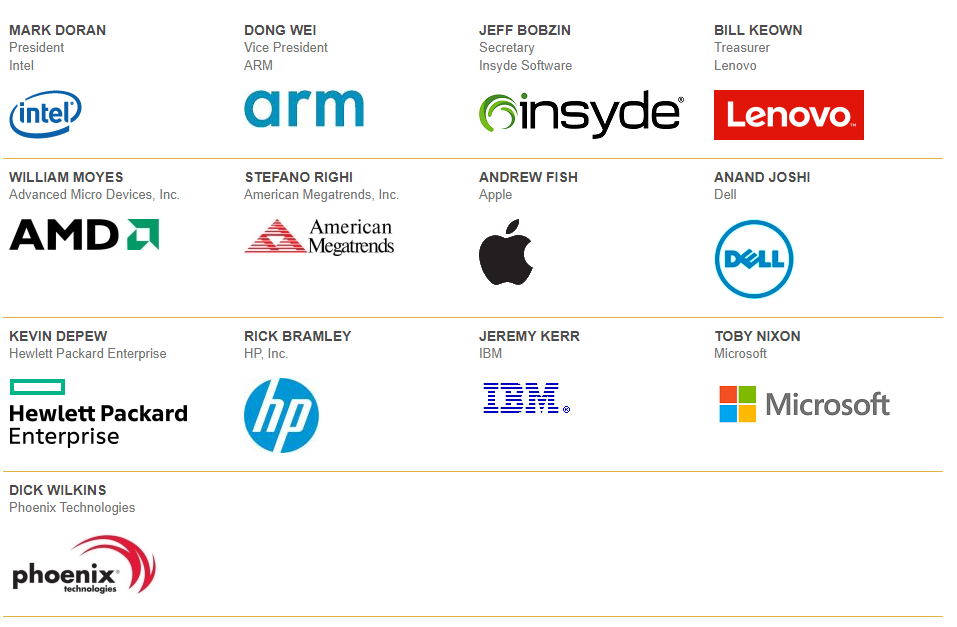
\includegraphics[width=\linewidth]{uefi_board_of_directors}
	\caption{Board of Directors of UEFI Forum}\label{fig:introduction-uefi-board-of-directors}
\end{figure}

The UEFI Forum board of directors consists of representatives from 11 industry leaders as described in Figure \ref{fig:introduction-uefi-board-of-directors}. These involved organizations work to ensure that the UEFI specifications meet industry needs.

UEFI uses a different interface for boot services and runtime services but UEFI does not specify how "Power On Self Test" (POST) and Setup are implemented - those are BIOS' primary functions.

\subsubsection{\gls{uefi} Driver Model Extension}
Access to boot devices is provided through a set of protocol interfaces. One purpose of the
UEFI Driver Model is to provide a replacement for \verb|PC-AT|-style option ROMs. It is important
to point out that drivers written to the UEFI Driver Model are designed to access boot devices in
the pre-boot environment. They are not designed to replace the high-performance, OS-specific
drivers.

The UEFI Driver Model is designed to support the execution of modular pieces of code,
also known as drivers, that run in the pre-boot environment. These drivers may manage or control
hardware buses and devices on the platform, or they may provide some software-derived, platform specific service. The UEFI Driver Model also contains information required by UEFI driver writers to design and implement any combination of bus drivers and device drivers that a platform
might need to boot a UEFI-compliant OS.

The UEFI Driver Model is designed to be generic and can be adapted to any type of bus or
device. The UEFI Specification describes how to write PCI bus drivers, PCI device drivers, USB
bus drivers, USB device drivers, and SCSI drivers. Additional details are provided that allow UEFI
drivers to be stored in PCI option ROMs, while maintaining compatibility with legacy option ROM
images.

One of the design goals in the UEFI Specification is keeping the driver images as small as
possible. However, if a driver is required to support multiple processor architectures, a driver
object file would also be required to be shipped for each supported processor architecture. To
address this space issue, this specification also defines the EFI Byte Code Virtual Machine. A
UEFI driver can be compiled into a single EFI Byte Code object file. UEFI Specificationcomplaint firmware must contain an EFI Byte Code interpreter. This allows a single EFI Byte
Code object file that supports multiple processor architectures to be shipped. Another space saving
technique is the use of compression. This specification defines compression and decompression
algorithms that may be used to reduce the size of UEFI Drivers, and thus reduce the overhead
when UEFI Drivers are stored in ROM devices.

The information contained in the UEFI Specification can be used by OSVs, IHVs, OEMs,
and firmware vendors to design and implement firmware conforming to this specification, drivers
that produce standard protocol interfaces, and operating system loaders that can be used to boot
UEFI compliant operating systems.

\subsubsection{\gls{uefi}'s Role in boot process}

During the boot process, UEFI speaks to the operating system loader and acts as the interface between the operating system and the BIOS.

The \verb|PC-AT| boot environment presents significant challenges to innovation within the
industry. Each new platform capability or hardware innovation requires firmware developers to
craft increasingly complex solutions, and often requires OS developers to make changes to their
boot code before customers can benefit from the innovation. This can be a time-consuming process
requiring a significant investment of resources. The primary goal of the UEFI specification is to
define an alternative boot environment that can alleviate some of these considerations. In this goal, the specification is like other existing boot specifications.

\subsection{Comparing of Legacy \gls{bios} and \gls{uefi}}

\begin{table}
	\centering
	\renewcommand{\arraystretch}{2}
	\caption{Legacy BIOS v/s UEFI}\label{table:legacy-bios-vs-uefi}
	\begin{tabular}{l | p{5cm} | p{5cm}}
		& Legacy BIOS & EFI
		\\ \hline \hline
		Language & Assembly & C ($ 99\% $)
		\\ \hline
		Resource & Interrupt Hardcode Memory Access hardcore I/O Access & Diver, Protocols
		\\ \hline
		Processor & x86 16-bit & CPU Protects Mode (Flat Mode)
		\\ \hline
		Expand & Hook Interrupt & Load Driver
		\\ \hline
		OS Bridge & ACPI & Run Time Driver Software
		\\ \hline
		$ 3^{rd} $ Party ISV \& IHV & Bas for Support & Easy for Support and for Multi Platforms
		\\ \hline
	\end{tabular}
\end{table}


\subsection{Advanced Configuration and Power Interface (\gls{acpi})}
The ACPI Component Architecture (ACPICA) defines and implements a group of software
components that together create an implementation of the ACPI specification. A major goal of the
architecture is to isolate all operating system dependencies to a relatively small translation or
conversion layer (the OS Services Layer) so that the bulk of the ACPICA code is independent of
any individual operating system. Therefore, hosting the ACPICA code on new operating systems
requires no source changes within the ACPICA code itself.

The components of the architecture include:
\begin{itemize}
	\item An OS-independent, kernel-resident ACPICA Subsystem component that provides the fundamental ACPI services such as the AML interpreter and namespace management.
	\item An OS-dependent OS Services Layer for each host operating system to provide OS support for the OS-independent ACPICA Subsystem.
	\item An ASL compiler-disassembler for translating ASL code to AML byte code and for disassembling existing binary ACPI tables back to ASL source code.
	\item Several ACPI utilities for executing the interpreter in ring 3 user space, extracting binary ACPI tables from the output of the ACPI Dump utility, and translating the ACPICA source	code to Linux/Unix format.
\end{itemize}

In Figure \ref{fig:introduction-acpi-component-architecture}, the ACPICA subsystem is shown in relation to the host operating system, device driver, OSPM software, and the ACPI hardware

\begin{figure}[h]
	\centering
	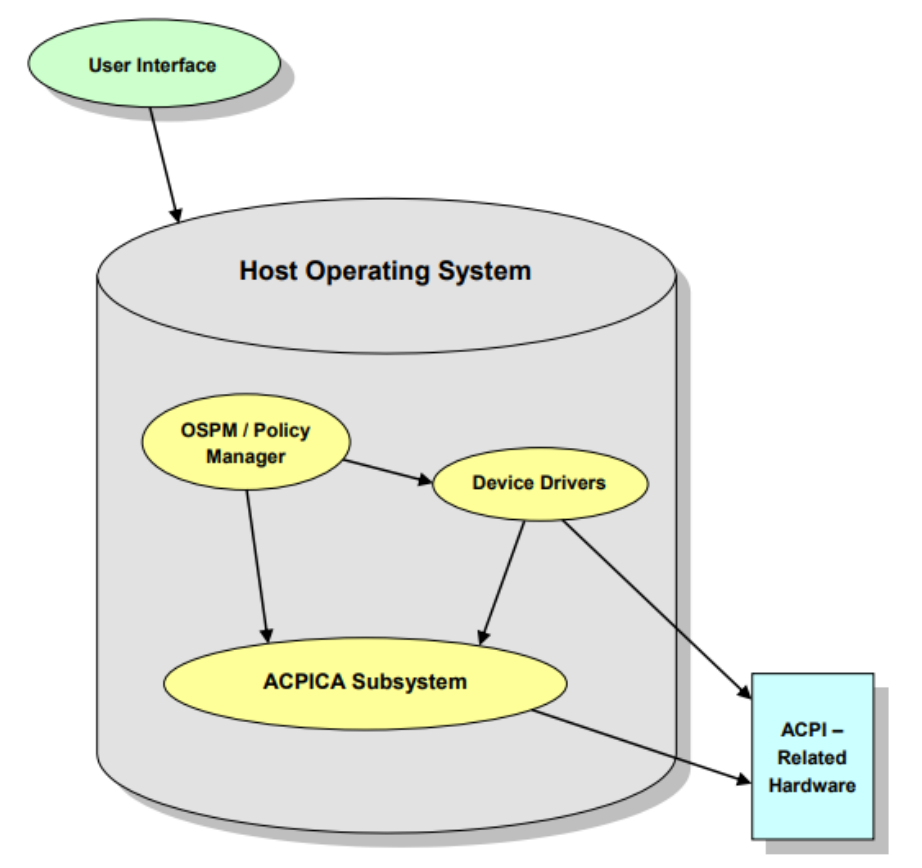
\includegraphics[width=0.7\linewidth]{introduction/acpi-component-architecture}
	\caption{The \gls{acpi} Component Architecture}\label{fig:introduction-acpi-component-architecture}
\end{figure}

\subsubsection{Overview of ACPICA Subsystem}
The ACPICA Subsystem implements the low level or fundamental aspects of the ACPI
specification. Included are an AML parser/interpreter, ACPI namespace management, ACPI table
and device support, and event handling. Since the ACPICA subsystem provides low-level system
services, it also requires low-level operating system services such as memory management,
synchronization, scheduling, and I/O.

To allow the ACPICA Subsystem to easily interface to any operating system that provides such
services, an Operating System Services Layer translates ACPICA-to-OS requests into the system
calls provided by the host operating system. The OS Services Layer is the only component of the
ACPICA that contains code that is specific to a host operating system.

Thus, the ACPICA Subsystem consists of two major software components:
\begin{itemize}
	\item The basic kernel-resident ACPICA Subsystem provides the fundamental ACPI services	that are independent of any particular operating system.
	\item The OS Services Layer (OSL) provides the conversion layer that interfaces the OS independent ACPICA Subsystem to a host operating system.
\end{itemize}

When combined into a single static or loadable software module such as a device driver or
kernel subsystem, these two major components form the ACPICA Subsystem. Throughout this
document, the term "ACPICA Subsystem" refers to the combination of the OS-independent
ACPICA Subsystem with an OS Services Layer components combined into a single module,
driver, or load unit.

\subsubsection{OS-independent ACPICA Subsystem}
The OS-independent ACPICA Subsystem supplies the major building blocks or subcomponents that are required for all ACPI implementations — including an AML interpreter, a namespace manager, ACPI event and resource management, and ACPI hardware support.

One of the goals of the ACPICA Subsystem is to provide an abstraction level high enough such
that the host operating system does not need to understand or know about the very low-level ACPI
details. For example, all AML code is hidden from the host. Also, the details of the ACPI hardware
are abstracted to higher-level software interfaces.

The ACPICA Subsystem implementation makes no assumptions about the host operating system or environment. The only way it can request operating system services is via interfaces provided by the OS Services Layer.

The primary user of the services provided by the ACPICA Subsystem are the host OS device drivers and power/thermal management software.

\subsubsection{Operating System Services Layer}
The OS Services Layer (or OSL) operates as a translation service for requests from the OS independent ACPICA subsystem back to the host OS. The OSL implements a generic set of OS service interfaces by using the primitives available from the host OS. Because of its nature.

The OS Services Layer must be implemented anew for each supported host operating
system. There is a single OS-independent ACPICA Subsystem, but there must be an OS Services
Layer for each operating system supported by the ACPI component architecture.

The primary function of the OSL in the ACPI Component Architecture is to be the small
glue layer that binds the much larger ACPICA Subsystem to the host operating system. Because
of the nature of ACPI itself — such as the requirement for an AML interpreter and management
of a large namespace data structure — most of the implementation of the ACPI specification is
independent of any operating system services. Therefore, the OS-independent ACPICA Subsystem
is the larger of the two components.

The overall ACPI Component Architecture in relation to the host operating system is Figure

\begin{figure}[h]
	\centering
	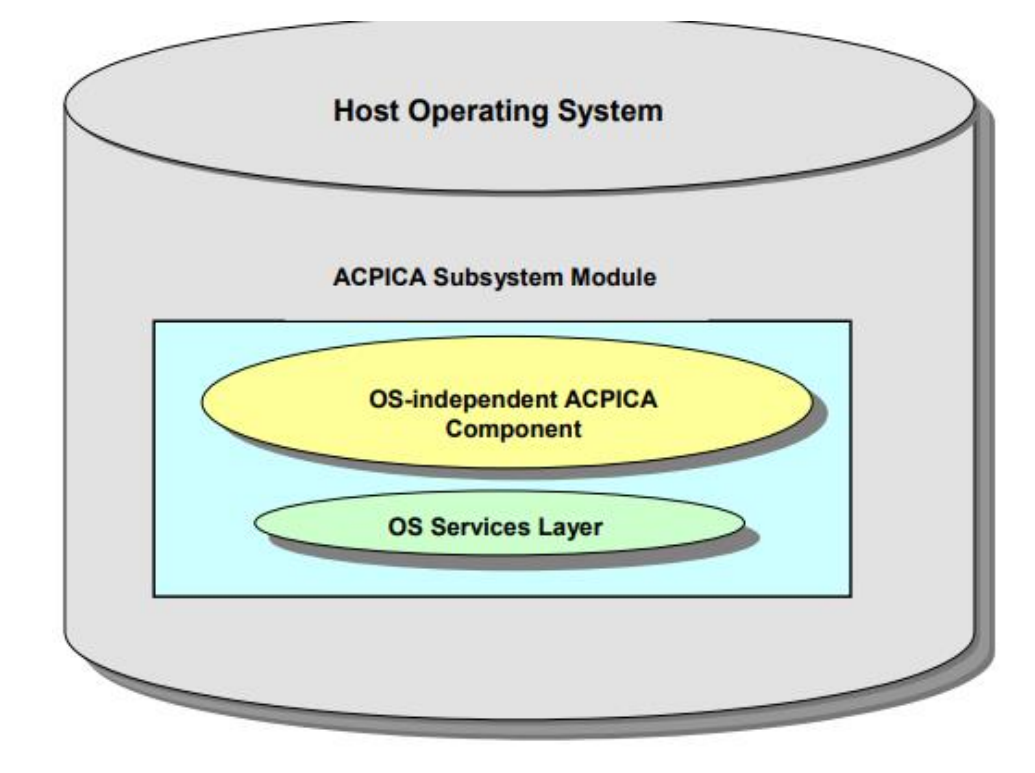
\includegraphics[width=0.7\linewidth]{introduction/acpica-subsystem-architecture}
	\caption{ACPICA Subsystem Architecture}\label{fig:introduction-acpica-subsystem-architecture}
\end{figure}

\subsubsection{ACPICA Subsystem Interaction}
The ACPICA Subsystem implements a set of external interfaces that can be directly called from
the host OS. These Acpi* interfaces provide the actual ACPI services for the host. When operating
system services are required during the servicing of an ACPI request, the Subsystem makes
requests to the host OS indirectly via the fixed AcpiOs* interfaces. The diagram below illustrates
the relationships and interaction between the various architectural elements by showing the flow
of control between them. Note that the OS-independent ACPICA Subsystem never calls the host directly instead it makes calls to the AcpiOs * interfaces in the OSL. This provides the ACPICA
code with OS-independence.

The Interaction between the Architectural Components Is shown in Figure \ref{fig:-introduction-acpi-interaction-between-the-architectural-components}

\begin{figure}[h]
	\centering
	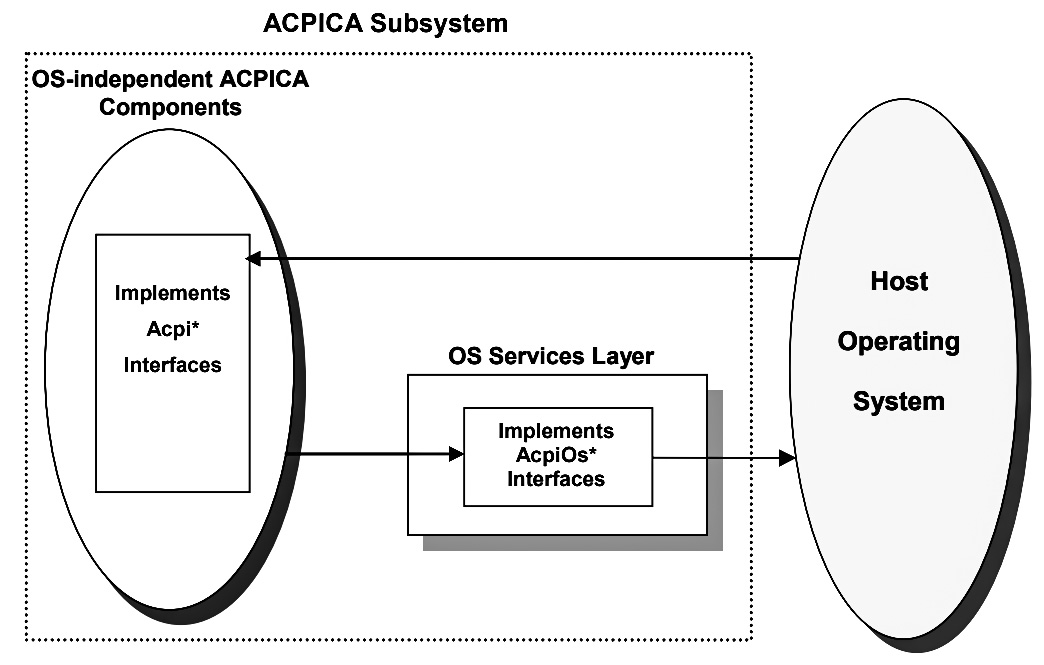
\includegraphics[width=0.7\linewidth]{introduction/acpi-interaction-between-the-architectural-components}
	\caption{Interaction between the Architectural Components}\label{fig:-introduction-acpi-interaction-between-the-architectural-components}
\end{figure}



\begin{frame}{BIOS: Basics}
    \begin{itemize}
        \item Set of Software Routines
            \begin{itemize}
                \item Initialize and test hardware on start
                \item Provides the OS with a generic hardware abstraction
            \end{itemize}
        \item the BIOS must do its job before your computer can load its operating system and applications
    \end{itemize}
\end{frame}

\begin{frame}{BIOS: Architecture}
    \begin{figure}
        \centering
        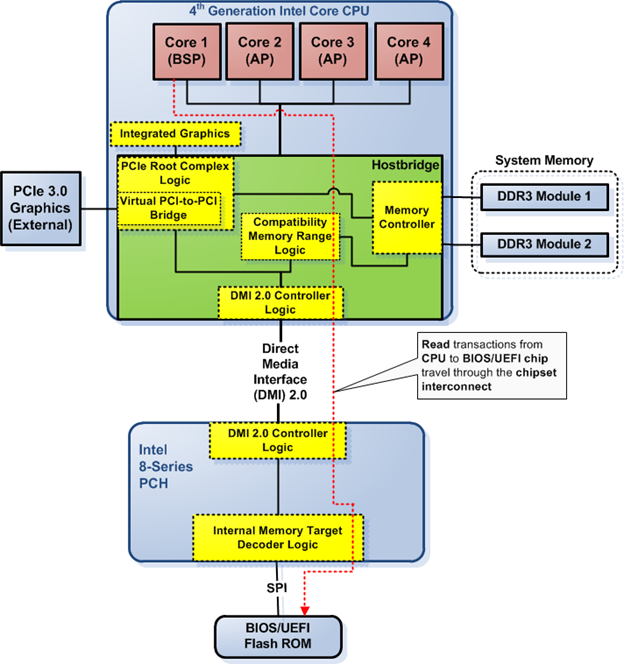
\includegraphics[width=0.6\linewidth]{Im/figures/bios-architecture.png}
        % \caption{BIOS Architecture}
        \label{fig:bios-architecture}
    \end{figure}
\end{frame}

\begin{frame}{BIOS: Firmware Image}
    \begin{figure}[htbp]
        \centering
        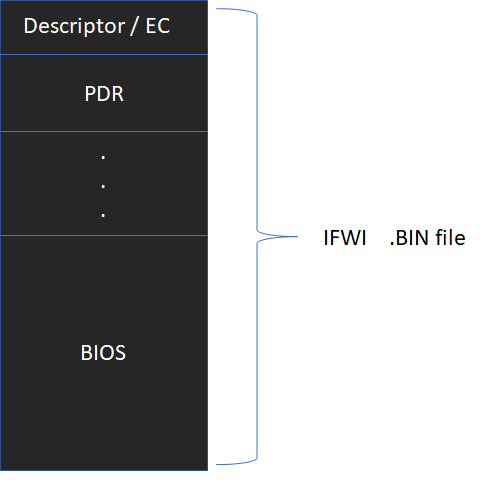
\includegraphics[width=0.6\linewidth]{Im/figures/design/integrated-firmware-image}
    \end{figure}
\end{frame}


\section{Requirement Specification}
\begin{frame}{Requirement Specification}
    \begin{itemize}
        \item Visual Studio C/C++ IDE
        \item Visual Studio Code
        \item Python 3
        \item Memory Access Interfaces\footnote{windows, linux, etc.}
    \end{itemize}
\end{frame}

\section{My Contribution}

\begin{frame}{My Contribution towards issues/challenges}
    \begin{figure}
        \centering
        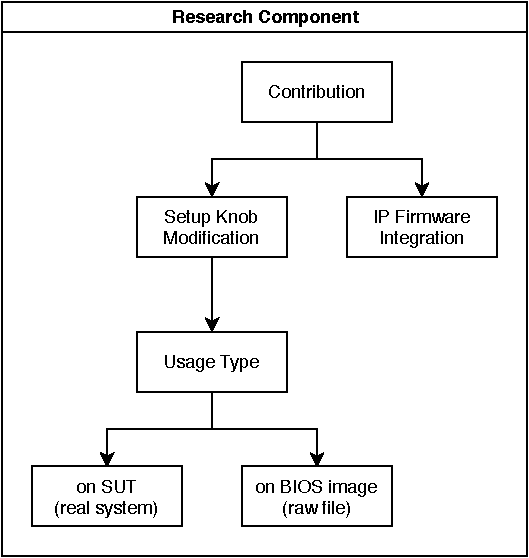
\includegraphics[width=0.6\linewidth]{Im/figures/research-component.pdf}
        % \caption{Research Component}
%        \label{fig:research-component}
    \end{figure}
\end{frame}

\begin{frame}[allowframebreaks]{Setup Knobs Modification: Process Flow}
    \begin{figure}[htbp]
        \centering
        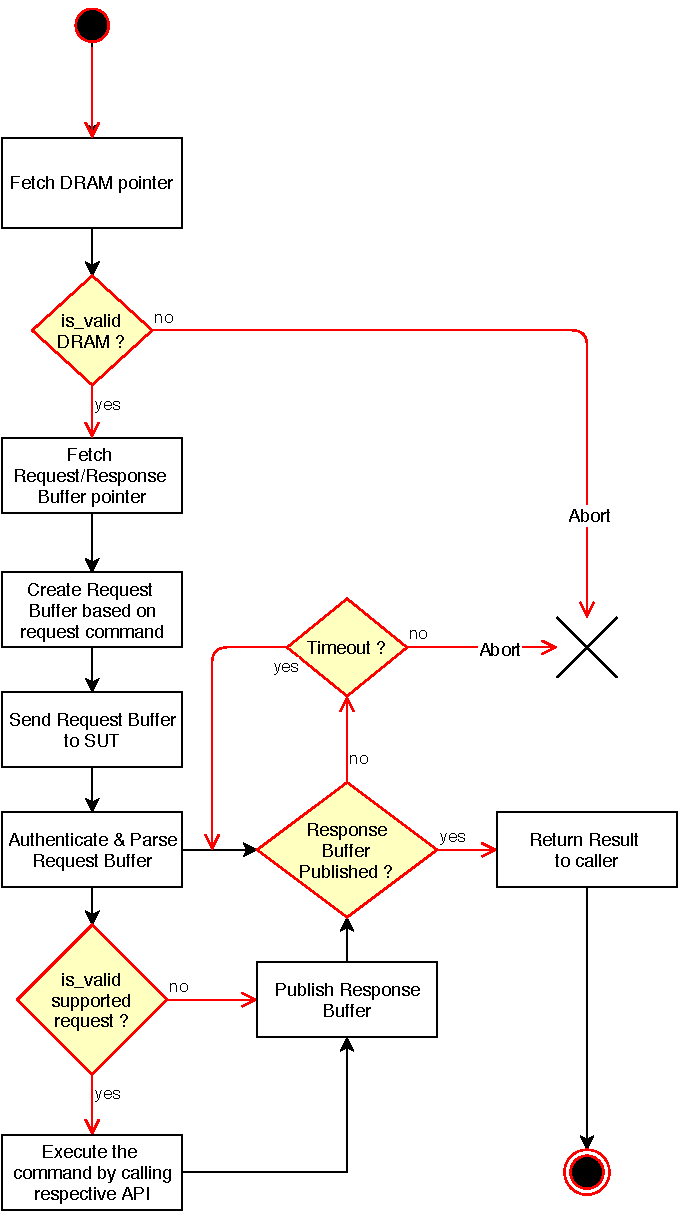
\includegraphics[width=0.3\linewidth]{Im/figures/setup-knobs-flow.pdf}
        \caption{Setup Knobs Modification Flow on SUT}
        \label{fig:setup-knobs-flow}
    \end{figure}
    
%    \begin{figure}[htbp]
%        \centering
%        \includegraphics[width=0.3\linewidth]{Im/figures/setup-knobs-flow-bios.pdf}
%        \caption{Setup Knobs Modification Flow on BIOS image}
%        \label{fig:setup-knobs-flow-bios}
%    \end{figure}
\end{frame}


\begin{frame}[allowframebreaks]{Setup Knobs Modification: Implementation Snaps}
    
    \begin{figure}[htbp]
        \centering
        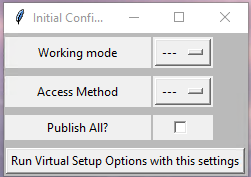
\includegraphics[width=0.6\linewidth]{Im/figures/proposed-work/bios-gui-initial-config}
        \caption{Menu to Select initial configuration for work}\label{fig:proposed-work-bios-gui-initial-config}
    \end{figure}
    
    \begin{figure}[htbp]
        \centering
        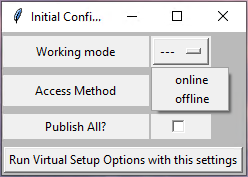
\includegraphics[width=0.6\linewidth]{Im/figures/proposed-work/bios-gui-initial-config-select-mode}
        \caption{Available work mode for the system: Online and Offline}\label{fig:proposed-work-bios-gui-initial-config-select-mode}
    \end{figure}

    \begin{figure}[htbp]
        \centering
        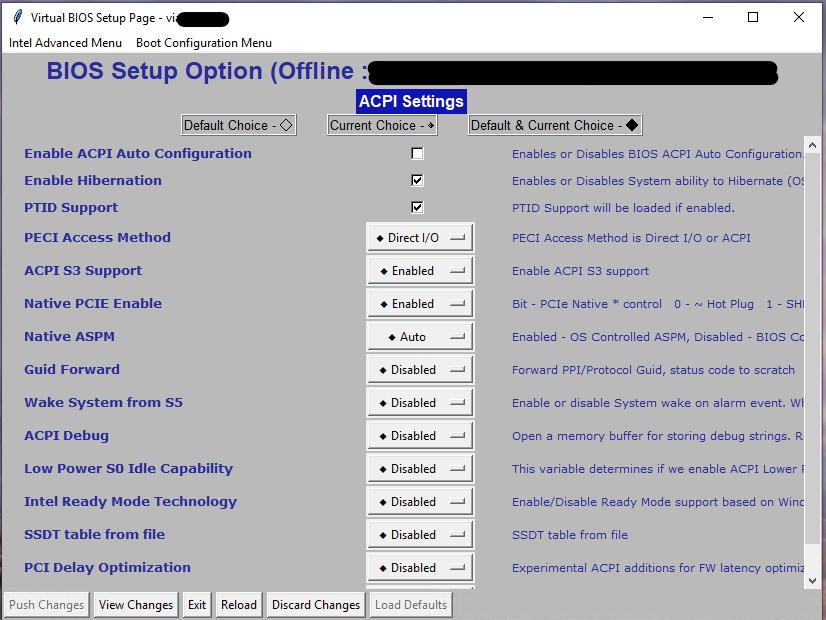
\includegraphics[width=0.6\linewidth]{Im/figures/proposed-work/bios-gui-acpi-knobs}
        \caption{Setup Options listed under ACPI Configurations}\label{fig:proposed-work-bios-gui-acpi-knobs}
    \end{figure}

    \begin{figure}[htbp]
        \centering
        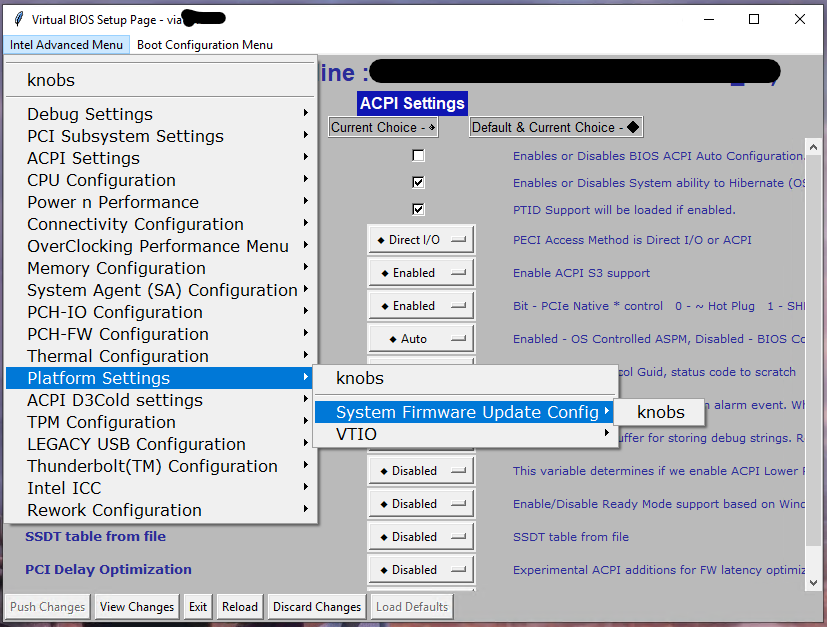
\includegraphics[width=0.6\linewidth]{Im/figures/proposed-work/bios-gui-accessing-menu}
        \caption{Navigating through BIOS setup page}\label{fig:proposed-work-bios-gui-accessing-menu}
    \end{figure}
\end{frame}

\begin{frame}{Setup Knobs Modification: Outcome}
    \begin{itemize}
        \item Cross platform usage
        \item API as a driver in BIOS Firmware
        \item Generic solution for usage types - on \textbf{SUT}, on \textbf{BIOS image}
        \item Information parsing and simulation
        \item Realtime sync for simulation changes
        \item Seamless Integration
    \end{itemize}
\end{frame}


\begin{frame}{IP firmware Integration: Structure of Module}
    \begin{figure}[htbp]
        \centering
        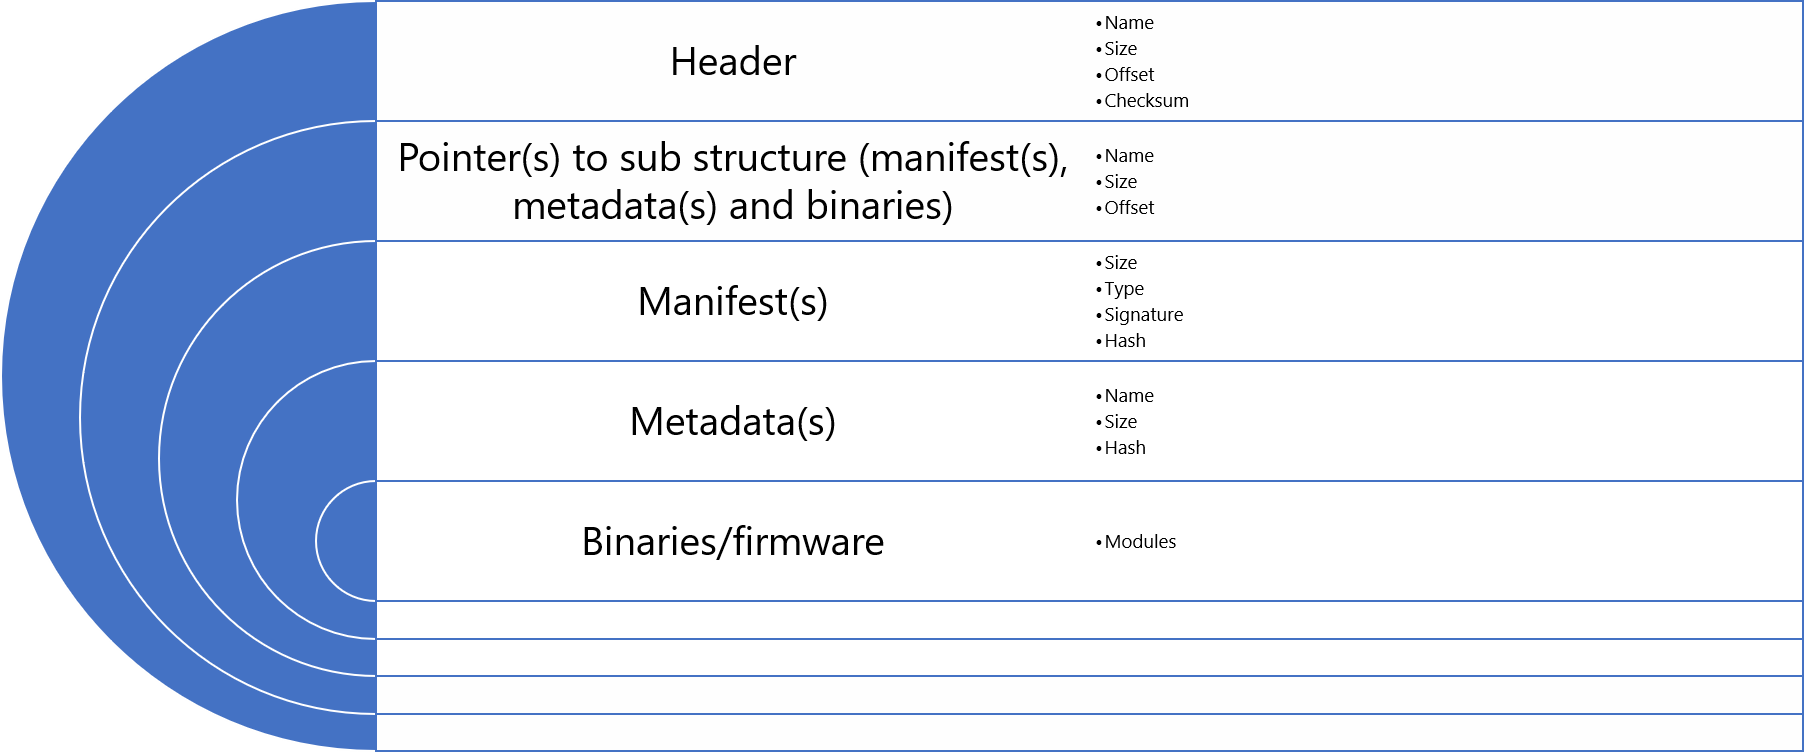
\includegraphics[width=0.9\linewidth]{Im/figures/proposed-work/proposed-structure-firmware-signing}
        \caption{Proposed Structure for firmware signing}\label{fig:proposed-work-proposed-structure-firmware-signing}
    \end{figure}
\end{frame}


\begin{frame}{IP firmware Integration: Outcome}
    \begin{itemize}
        \item Removal of IP dependency during firmware loading
        \item IP Subsystem :
        \begin{itemize}
            \item Loader and Verifier
            \item IP is always consumer
        \end{itemize}
        \item Signature verification using SHA hash algorithm
        \item Seamless Integration of any other hash algorithm for verification
        \item Hardware based and Software based verification support
        \item Prevent common security threats
        \item Allow easier OEM adoption and modification based on the respective design
        \item Reusability/Portability of design across many IPs
        \item Generic design which supports any new IP integration
    \end{itemize}
\end{frame}

\section{Future Scope}
\begin{frame}{Future Scope}
    \begin{itemize}
      \item Development and testing of individual driver component rather than building the whole BIOS image
      \item AI powered Search Engine to enhance the findings of FAQs for relevant existing queries and articles
      \item Automating the initial BIOS Environment Setup
      \item Platform independent easy installation setup for the framework
    \end{itemize}
\end{frame}

\section{Phase 1: Study of existing architecture for hotspot}
\begin{frame}{Phase 1: Study of existing architecture for hotspot}
	\begin{itemize}
		\item Identifying changes of two different BIOS Image of different check-ins
		\item Lookup of module by GUID and vice-versa
		\item Exposed source code support for OEM information
		\item Runtime BIOS Support for temporary UEFI variable creation		
	\end{itemize}
\end{frame}

\section{Phase 2: Analysis and gathering detailed information of the problem}
\begin{frame}{Phase 2: Analysis and gathering detailed information of the problem}
	\begin{itemize}
		\item Debugging via comparing Setup Knobs
		\item Lookup of order of the module in BIOS Image as file system
		\item Verification of module integration via GUID
		\item OEM needs to fill information which need not to compulsorily expose the source code
		\item Automation and Testing for \textbf{non-BIOS driver} require BIOS Support for creation of temporary UEFI variables 
	\end{itemize}
\end{frame}

\section{Requirement Specification}
\begin{frame}{Requirement Specification}
\end{frame}

\section{Why JSON?}
\begin{frame}{Why JSON?}
	
\end{frame}

\section{Implementation of Parsing}
%\begin{frame}{Implementation of Parsing}
%	Flow diagram of BIOS Image parsing
%\end{frame} 

\begin{frame}{Implementation of Parsing: Format of BIOS Image}
	\begin{figure}[htbp]
		\centering
		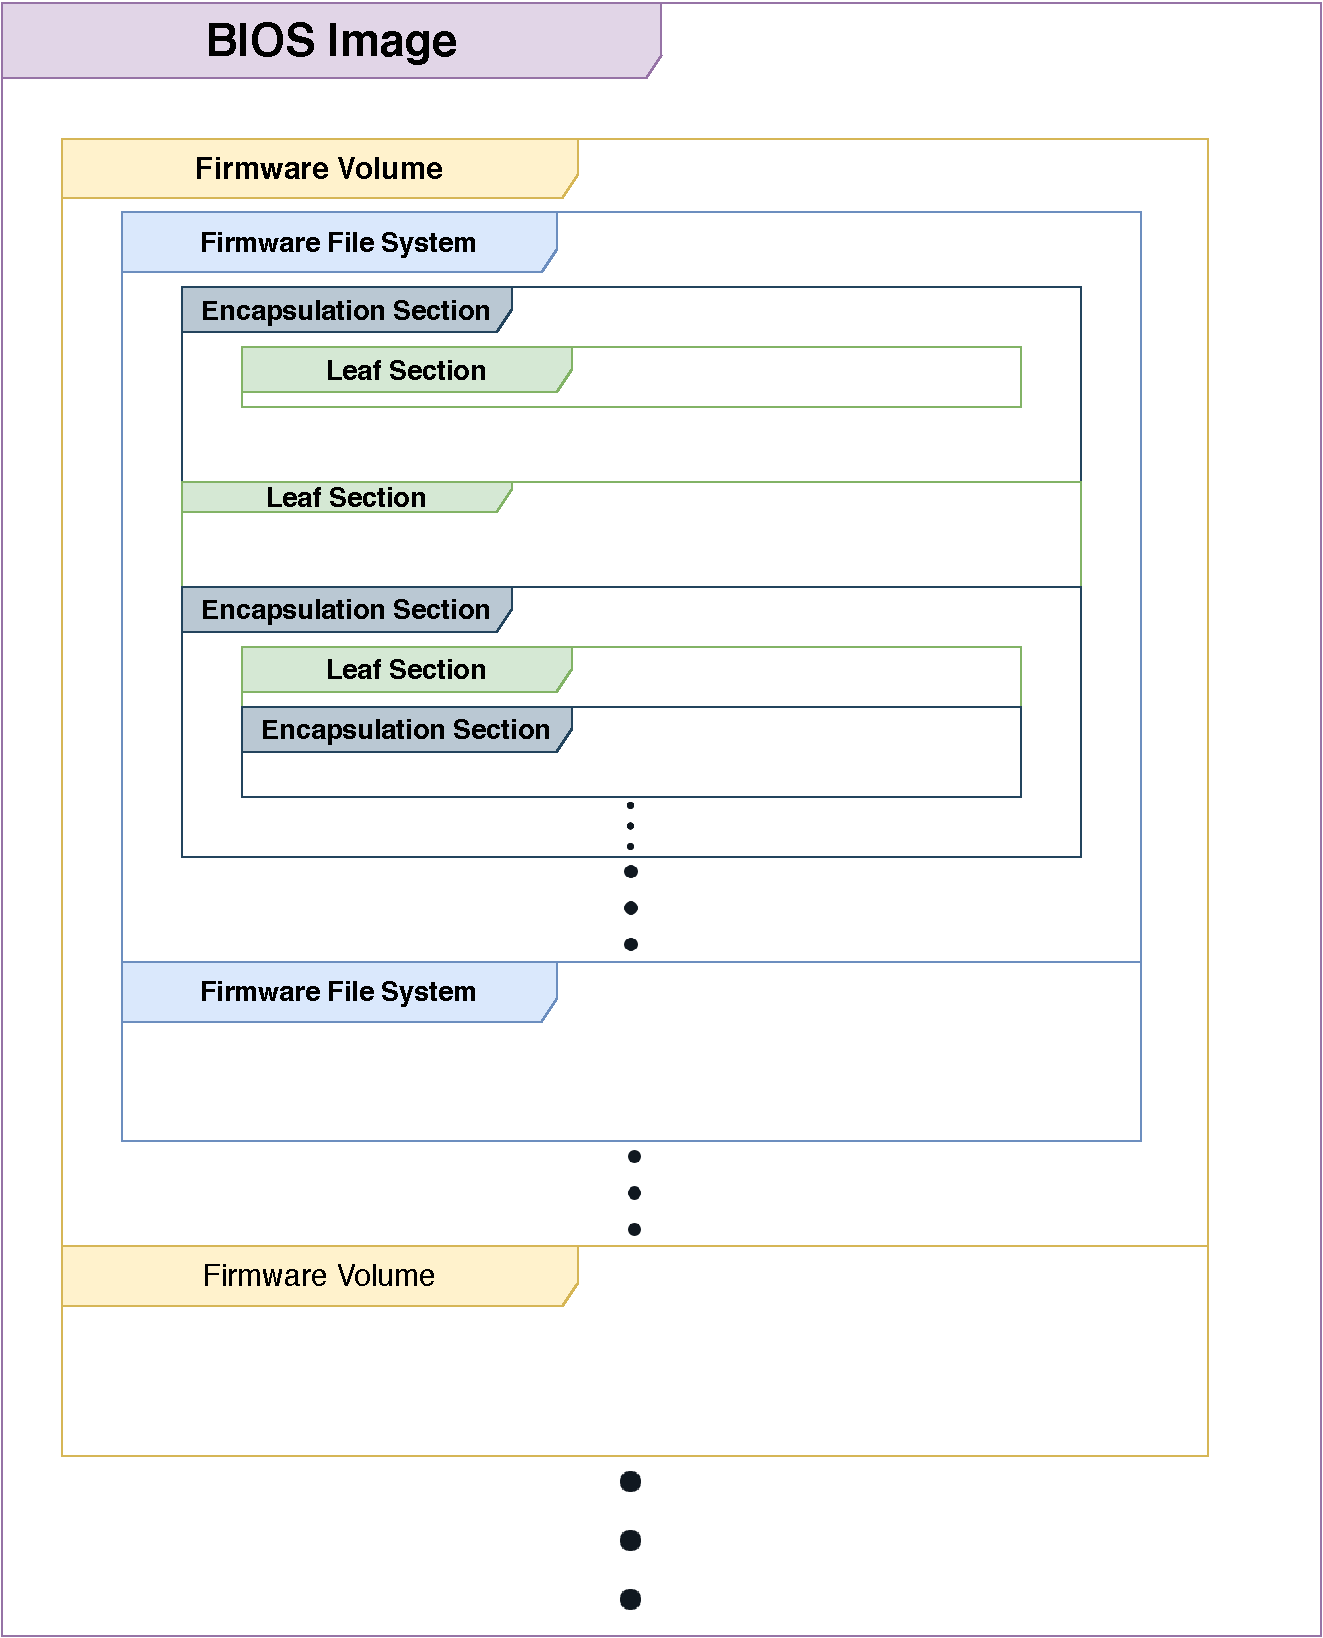
\includegraphics[width=0.5\linewidth]{Im/figures/bios-as-filesystem.pdf}
%		\caption{Each Firmware Volume in BIOS Image}
%		\label{fig:the-firmware-volume-format}
	\end{figure}
\end{frame}

\begin{frame}{Implementation of Parsing: Work Flow}
	\begin{figure}[htbp]
		\centering
		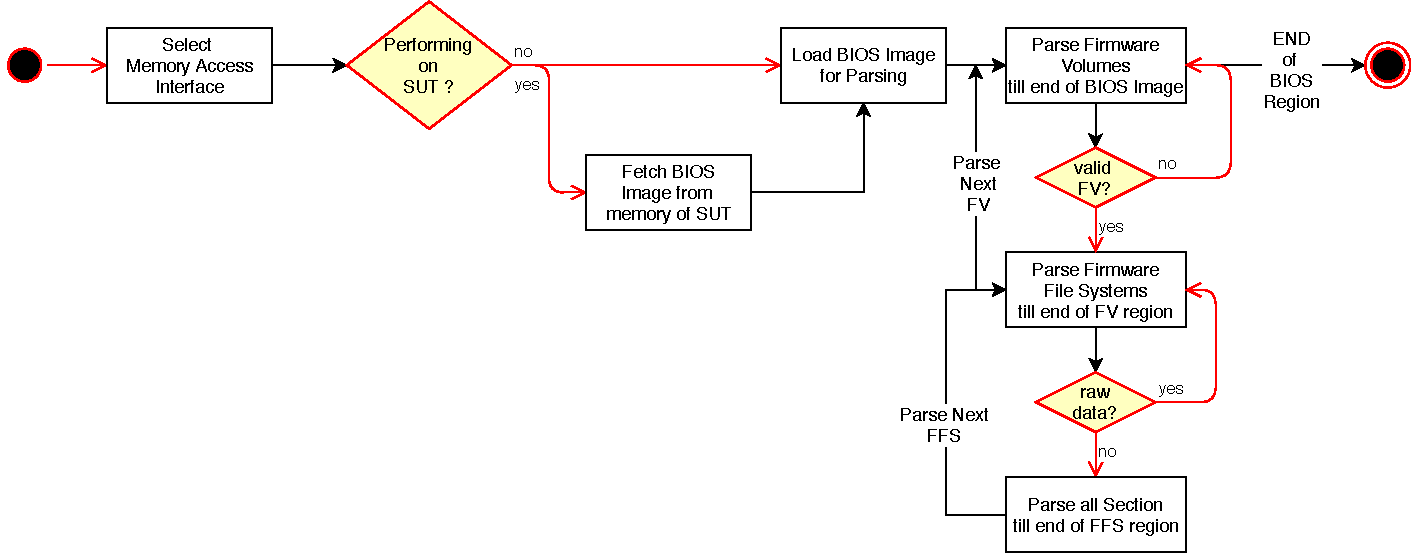
\includegraphics[width=\linewidth]{Im/figures/uefi-parser.pdf}
		%		\caption{Each Firmware Volume in BIOS Image}
		%		\label{fig:uefi-parser-flow}
	\end{figure}
\end{frame}

\begin{frame}{Outcome}
	\begin{itemize}
		\item Human Readable interpretation of BIOS Image
		\item GUIDs Lookup
		\item Verification of existence of module by GUID
		\item Storing the image file system content by GUID
		\item Summarizing changes of two BIOS image
	\end{itemize}
\end{frame}

% Here begins the new contents.......


% \section{Awards}
% \begin{frame}{Awards}
    \begin{figure}[htbp]
        \centering
        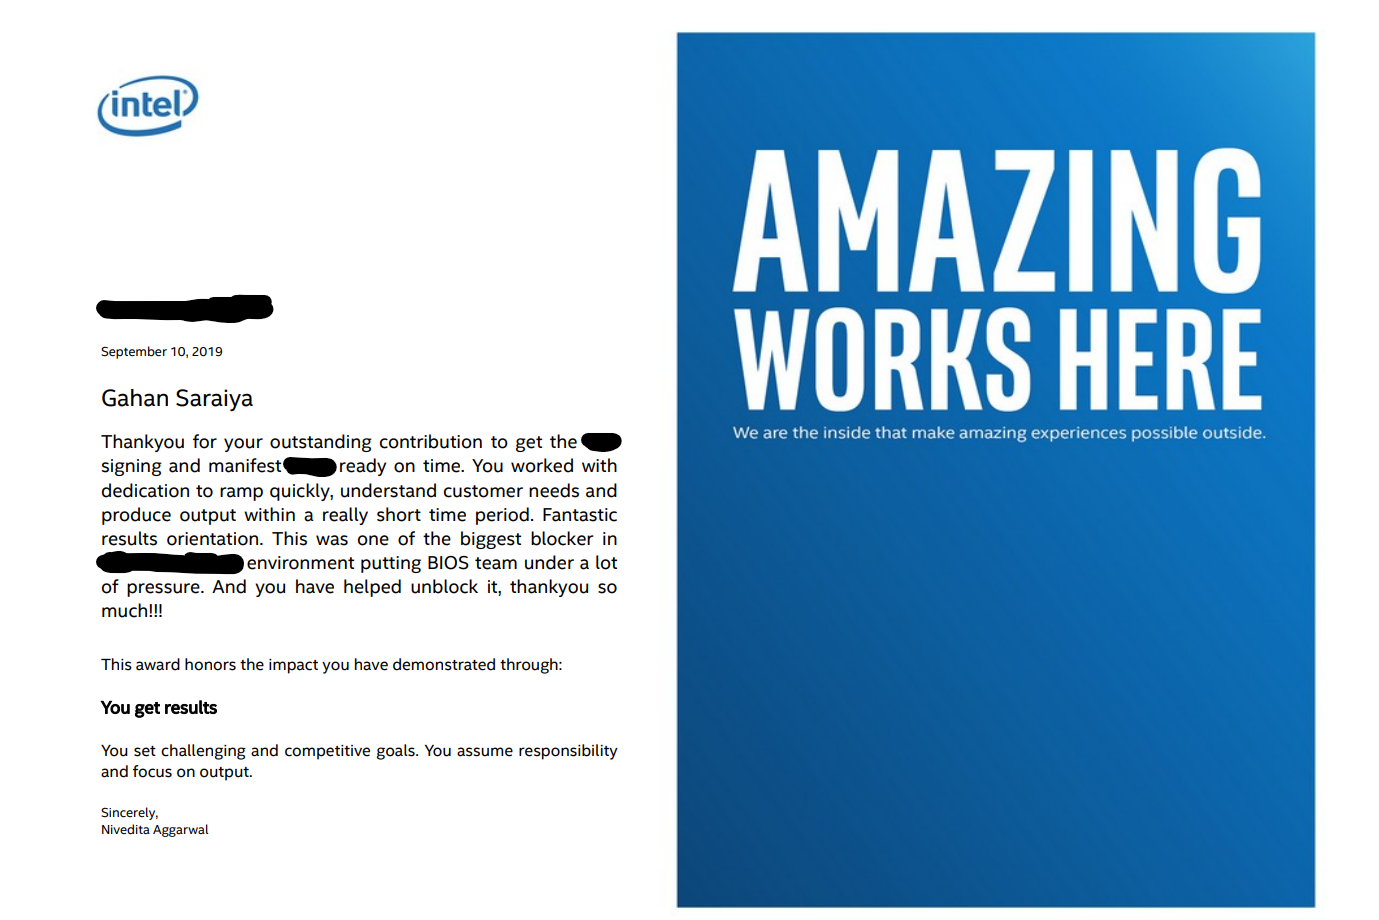
\includegraphics[width=\linewidth]{Im/figures/award1}
    \end{figure}
\end{frame}


%\nocite{*}
%\begin{frame}[plain, noframenumbering,allowframebreaks]{References}
%    \printbibliography
%\end{frame}


%\appendix

%\section*{Appendix A}

\begin{frame}{Appendix slide number 1}
    \lipsum[1]
\end{frame}

\section*{Appendix B}

\begin{frame}{Appendix slide number 2}
    \lipsum[2]
\end{frame}
\section*{}
\begin{frame}{}
	\centering \Huge
	\emph{Thank You}
\end{frame}

\end{document}